\documentclass[12pt,]{article}
\usepackage{lmodern}
\usepackage{amssymb,amsmath}
\usepackage{ifxetex,ifluatex}
\usepackage{fixltx2e} % provides \textsubscript
\ifnum 0\ifxetex 1\fi\ifluatex 1\fi=0 % if pdftex
  \usepackage[T1]{fontenc}
  \usepackage[utf8]{inputenc}
\else % if luatex or xelatex
  \ifxetex
    \usepackage{mathspec}
  \else
    \usepackage{fontspec}
  \fi
  \defaultfontfeatures{Ligatures=TeX,Scale=MatchLowercase}
    \setmainfont[]{Times New Roman}
\fi
% use upquote if available, for straight quotes in verbatim environments
\IfFileExists{upquote.sty}{\usepackage{upquote}}{}
% use microtype if available
\IfFileExists{microtype.sty}{%
\usepackage{microtype}
\UseMicrotypeSet[protrusion]{basicmath} % disable protrusion for tt fonts
}{}
\usepackage[margin=2.54cm]{geometry}
\usepackage{hyperref}
\hypersetup{unicode=true,
            pdftitle={Assessing phytoplankton abundance in North Temperate Lakes},
            pdfauthor={Siying Chen},
            pdfborder={0 0 0},
            breaklinks=true}
\urlstyle{same}  % don't use monospace font for urls
\usepackage{color}
\usepackage{fancyvrb}
\newcommand{\VerbBar}{|}
\newcommand{\VERB}{\Verb[commandchars=\\\{\}]}
\DefineVerbatimEnvironment{Highlighting}{Verbatim}{commandchars=\\\{\}}
% Add ',fontsize=\small' for more characters per line
\usepackage{framed}
\definecolor{shadecolor}{RGB}{248,248,248}
\newenvironment{Shaded}{\begin{snugshade}}{\end{snugshade}}
\newcommand{\KeywordTok}[1]{\textcolor[rgb]{0.13,0.29,0.53}{\textbf{#1}}}
\newcommand{\DataTypeTok}[1]{\textcolor[rgb]{0.13,0.29,0.53}{#1}}
\newcommand{\DecValTok}[1]{\textcolor[rgb]{0.00,0.00,0.81}{#1}}
\newcommand{\BaseNTok}[1]{\textcolor[rgb]{0.00,0.00,0.81}{#1}}
\newcommand{\FloatTok}[1]{\textcolor[rgb]{0.00,0.00,0.81}{#1}}
\newcommand{\ConstantTok}[1]{\textcolor[rgb]{0.00,0.00,0.00}{#1}}
\newcommand{\CharTok}[1]{\textcolor[rgb]{0.31,0.60,0.02}{#1}}
\newcommand{\SpecialCharTok}[1]{\textcolor[rgb]{0.00,0.00,0.00}{#1}}
\newcommand{\StringTok}[1]{\textcolor[rgb]{0.31,0.60,0.02}{#1}}
\newcommand{\VerbatimStringTok}[1]{\textcolor[rgb]{0.31,0.60,0.02}{#1}}
\newcommand{\SpecialStringTok}[1]{\textcolor[rgb]{0.31,0.60,0.02}{#1}}
\newcommand{\ImportTok}[1]{#1}
\newcommand{\CommentTok}[1]{\textcolor[rgb]{0.56,0.35,0.01}{\textit{#1}}}
\newcommand{\DocumentationTok}[1]{\textcolor[rgb]{0.56,0.35,0.01}{\textbf{\textit{#1}}}}
\newcommand{\AnnotationTok}[1]{\textcolor[rgb]{0.56,0.35,0.01}{\textbf{\textit{#1}}}}
\newcommand{\CommentVarTok}[1]{\textcolor[rgb]{0.56,0.35,0.01}{\textbf{\textit{#1}}}}
\newcommand{\OtherTok}[1]{\textcolor[rgb]{0.56,0.35,0.01}{#1}}
\newcommand{\FunctionTok}[1]{\textcolor[rgb]{0.00,0.00,0.00}{#1}}
\newcommand{\VariableTok}[1]{\textcolor[rgb]{0.00,0.00,0.00}{#1}}
\newcommand{\ControlFlowTok}[1]{\textcolor[rgb]{0.13,0.29,0.53}{\textbf{#1}}}
\newcommand{\OperatorTok}[1]{\textcolor[rgb]{0.81,0.36,0.00}{\textbf{#1}}}
\newcommand{\BuiltInTok}[1]{#1}
\newcommand{\ExtensionTok}[1]{#1}
\newcommand{\PreprocessorTok}[1]{\textcolor[rgb]{0.56,0.35,0.01}{\textit{#1}}}
\newcommand{\AttributeTok}[1]{\textcolor[rgb]{0.77,0.63,0.00}{#1}}
\newcommand{\RegionMarkerTok}[1]{#1}
\newcommand{\InformationTok}[1]{\textcolor[rgb]{0.56,0.35,0.01}{\textbf{\textit{#1}}}}
\newcommand{\WarningTok}[1]{\textcolor[rgb]{0.56,0.35,0.01}{\textbf{\textit{#1}}}}
\newcommand{\AlertTok}[1]{\textcolor[rgb]{0.94,0.16,0.16}{#1}}
\newcommand{\ErrorTok}[1]{\textcolor[rgb]{0.64,0.00,0.00}{\textbf{#1}}}
\newcommand{\NormalTok}[1]{#1}
\usepackage{longtable,booktabs}
\usepackage{graphicx,grffile}
\makeatletter
\def\maxwidth{\ifdim\Gin@nat@width>\linewidth\linewidth\else\Gin@nat@width\fi}
\def\maxheight{\ifdim\Gin@nat@height>\textheight\textheight\else\Gin@nat@height\fi}
\makeatother
% Scale images if necessary, so that they will not overflow the page
% margins by default, and it is still possible to overwrite the defaults
% using explicit options in \includegraphics[width, height, ...]{}
\setkeys{Gin}{width=\maxwidth,height=\maxheight,keepaspectratio}
\IfFileExists{parskip.sty}{%
\usepackage{parskip}
}{% else
\setlength{\parindent}{0pt}
\setlength{\parskip}{6pt plus 2pt minus 1pt}
}
\setlength{\emergencystretch}{3em}  % prevent overfull lines
\providecommand{\tightlist}{%
  \setlength{\itemsep}{0pt}\setlength{\parskip}{0pt}}
\setcounter{secnumdepth}{5}
% Redefines (sub)paragraphs to behave more like sections
\ifx\paragraph\undefined\else
\let\oldparagraph\paragraph
\renewcommand{\paragraph}[1]{\oldparagraph{#1}\mbox{}}
\fi
\ifx\subparagraph\undefined\else
\let\oldsubparagraph\subparagraph
\renewcommand{\subparagraph}[1]{\oldsubparagraph{#1}\mbox{}}
\fi

%%% Use protect on footnotes to avoid problems with footnotes in titles
\let\rmarkdownfootnote\footnote%
\def\footnote{\protect\rmarkdownfootnote}

%%% Change title format to be more compact
\usepackage{titling}

% Create subtitle command for use in maketitle
\newcommand{\subtitle}[1]{
  \posttitle{
    \begin{center}\large#1\end{center}
    }
}

\setlength{\droptitle}{-2em}

  \title{Assessing phytoplankton abundance in North Temperate Lakes}
    \pretitle{\vspace{\droptitle}\centering\huge}
  \posttitle{\par}
  \subtitle{\url{https://github.com/Sylvia-C/872_Final.git}}
  \author{Siying Chen}
    \preauthor{\centering\large\emph}
  \postauthor{\par}
    \date{}
    \predate{}\postdate{}
  

\begin{document}
\maketitle
\begin{abstract}
Phytoplankton growth depends on the availability of carbon dioxide,
sunlight, and nutrients. This project uses data from studies on several
lakes in the North Temperate Lakes District in Wisconsin, USA as part of
the Long Term Ecological Research station established by the National
Science Foundation. The purpose of this project is to find out the
relationship between phytoplankton abundance (biovolume) and nutrients
(nitrogen and phosphorus) using regression analysis. There are 2
datasets used in this project, which are the nutrients dataset and
phytoplankton dataset of the lakes.
\end{abstract}

\newpage

\tableofcontents  \newpage
\listoftables 

\newpage

\listoffigures 
{r Figure 1, echo =F, fig.cap="x"}
{r Figure 2, echo =F, fig.cap="x"}
{r Figure 3, echo =F, fig.cap="x"}
{r Figure 4, echo =F, fig.cap="x"}
{r Figure 5, echo =F, fig.cap="x"}
{r Figure 6, echo =F, fig.cap="x"} \newpage

\textless{}Note: set up autoreferencing for figures and tables in your
document\textgreater{}

\section{Research Question and
Rationale}\label{research-question-and-rationale}

Phytoplankton growth depends on the availability of carbon dioxide,
sunlight, and nutrients. Like other plants, phytoplanktons require
nutrients like nitrogen and phosphorus to survive. In this project, I
would like to look at total nitrogen and total phosphorus concentration
and see how they interact with phytoplankton abundance, which was
measured in biovolume. This project can help peole to understand the
relationship between phytoplankton growth and the concentration of
nutrients like nitrogen and phosphorus at North Temperate Lakes.

Due to data availability, we will only be looking at East Long Lake,
Paul Lake, Peter Lake, Tuesday Lake, and West Long Lake. For this
project, I'll be focusing on the division level of phytoplankton
abundance, which are measured in biovolume in millimeter cubed per
liter. I'll sum up the total biovolume of different phytoplankton
division at each lake on each data. For nutrients data, since the
nutrient concentration was collected at different depth, I'll use the
median concentration for each lake on each date to avoid outliers. The
research question for this project are: 1. How total nitrogen
concentration affect the abundance of phytoplankton in these 5 lakes? 2.
How total phosphorus concentration affect the abundance of phytoplankton
in these 5 lakes?

\newpage

\section{Dataset Information}\label{dataset-information}

Nutrient data were collected from 1991-2016. They are usually collected
in the morning and collected at different depth. Chemical measurements
are collected in several ways: pooled mixed layer sample (PML),
epilimnion, metalimnion, and hypolimnion, or vertical profiles. On each
sampling date, there are up to seven samples due to Van Dorn collections
across a depth interval according to percent irradiance. Nutrient
samples were sent to the Cary Institute of Ecosystem Studies for
analysis beginning in 2000. The Kjeldahl method for measuring nitrogen
is not used at IES, and so measurements reported from 2000 onwards are
Total Nitrogen.

Data on epilimnetic phytoplankton were collected from 1984-2015,
determined by light microscopy from pooled Van Dorn samples at 100
percent, 50 percent, and 25 percent of surface irradiance. Samples
collected after 1995 were counted by Phycotech Inc. Sampling were
conducted at 5 lakes and the frequency varies. Data include taxonomic
information and split into distinct columns of genus, species and
description for archival as best possible.

\begin{longtable}[]{@{}lll@{}}
\toprule
\begin{minipage}[b]{0.13\columnwidth}\raggedright\strut
Dataset\strut
\end{minipage} & \begin{minipage}[b]{0.54\columnwidth}\raggedright\strut
Data Column\strut
\end{minipage} & \begin{minipage}[b]{0.24\columnwidth}\raggedright\strut
Unit\strut
\end{minipage}\tabularnewline
\midrule
\endhead
\begin{minipage}[t]{0.13\columnwidth}\raggedright\strut
Nutrients\strut
\end{minipage} & \begin{minipage}[t]{0.54\columnwidth}\raggedright\strut
Total nitrogen concentration, total phosphorus concentration\strut
\end{minipage} & \begin{minipage}[t]{0.24\columnwidth}\raggedright\strut
Micrograms Per Liter\strut
\end{minipage}\tabularnewline
\begin{minipage}[t]{0.13\columnwidth}\raggedright\strut
Phytoplankton\strut
\end{minipage} & \begin{minipage}[t]{0.54\columnwidth}\raggedright\strut
Total biovolume\strut
\end{minipage} & \begin{minipage}[t]{0.24\columnwidth}\raggedright\strut
Millimeter Cubed Per Liter\strut
\end{minipage}\tabularnewline
\bottomrule
\end{longtable}

\newpage

\section{Exploratory Data Analysis and
Wrangling}\label{exploratory-data-analysis-and-wrangling}

\begin{Shaded}
\begin{Highlighting}[]
\CommentTok{# Read in datasets as dataframe}
\NormalTok{nutrients <-}\StringTok{ }\KeywordTok{read.csv}\NormalTok{(}\StringTok{"./Raw/NTL-LTER_Lake_Nutrients_Raw.csv"}\NormalTok{)}
\NormalTok{phytoplankton <-}\StringTok{ }\KeywordTok{read.csv}\NormalTok{(}\StringTok{"./Raw/NTL-LTER_Lake_Phytoplankton_Raw.csv"}\NormalTok{)}

\CommentTok{# Format sampledate as date}
\NormalTok{nutrients}\OperatorTok{$}\NormalTok{sampledate <-}\StringTok{ }
\StringTok{  }\KeywordTok{as.Date}\NormalTok{(nutrients}\OperatorTok{$}\NormalTok{sampledate, }\DataTypeTok{format =} \StringTok{"%m/%d/%y"}\NormalTok{)}
\NormalTok{phytoplankton}\OperatorTok{$}\NormalTok{sampledate <-}\StringTok{ }
\StringTok{  }\KeywordTok{as.Date}\NormalTok{(phytoplankton}\OperatorTok{$}\NormalTok{sampledate, }\DataTypeTok{format =} \StringTok{"%Y-%m-%d"}\NormalTok{)}

\CommentTok{# Select and filter dataframe to slim the data}
\NormalTok{nutrients_slim <-}\StringTok{ }\NormalTok{nutrients }\OperatorTok
\StringTok{  }\KeywordTok{select}\NormalTok{(lakename, sampledate, depth, tn_ug, tp_ug) }\OperatorTok
\StringTok{  }\KeywordTok{na.omit}\NormalTok{() }\OperatorTok
\StringTok{  }\KeywordTok{group_by}\NormalTok{(lakename, sampledate) }\OperatorTok
\StringTok{  }\KeywordTok{summarize}\NormalTok{(}\DataTypeTok{medianTN =} \KeywordTok{median}\NormalTok{(tn_ug),}
            \DataTypeTok{medianTP =} \KeywordTok{median}\NormalTok{(tp_ug))}

\NormalTok{phytoplankton_slim <-}\StringTok{ }\NormalTok{phytoplankton }\OperatorTok
\StringTok{  }\KeywordTok{select}\NormalTok{(lakename, sampledate, division, total_biovol) }\OperatorTok
\StringTok{  }\KeywordTok{group_by}\NormalTok{(lakename, sampledate, division) }\OperatorTok
\StringTok{  }\KeywordTok{summarize}\NormalTok{(}\DataTypeTok{biomass =} \KeywordTok{sum}\NormalTok{(total_biovol))}

\CommentTok{# Join datasets}
\NormalTok{biomass_nutrients <-}\StringTok{ }\NormalTok{phytoplankton_slim }\OperatorTok
\StringTok{  }\KeywordTok{summarize}\NormalTok{(}\DataTypeTok{tot_biomass =} \KeywordTok{sum}\NormalTok{(biomass)) }\OperatorTok
\StringTok{  }\KeywordTok{left_join}\NormalTok{(nutrients_slim, }\DataTypeTok{by =} \KeywordTok{c}\NormalTok{(}\StringTok{"lakename"}\NormalTok{ =}\StringTok{ "lakename"}\NormalTok{, }\StringTok{"sampledate"}\NormalTok{ =}\StringTok{ "sampledate"}\NormalTok{)) }\OperatorTok
\StringTok{  }\KeywordTok{na.omit}\NormalTok{()}
\end{Highlighting}
\end{Shaded}

\begin{verbatim}
## Warning: Column `lakename` joining factors with different levels, coercing
## to character vector
\end{verbatim}

\begin{Shaded}
\begin{Highlighting}[]
\CommentTok{#colnames(biomass_nutrients) <- c("Lake Name", "Sample Date", "Biomass", "Median TN", "Median TP")}

\CommentTok{# Summary statistics}
\KeywordTok{head}\NormalTok{(phytoplankton_slim)}
\end{Highlighting}
\end{Shaded}

\begin{verbatim}
## # A tibble: 6 x 4
## # Groups:   lakename, sampledate [1]
##   lakename       sampledate division        biomass
##   <fct>          <date>     <fct>             <dbl>
## 1 East Long Lake 1989-05-26 Bacillariophyta   0.012
## 2 East Long Lake 1989-05-26 Chlorophyta       0.012
## 3 East Long Lake 1989-05-26 Chrysophyta       0.304
## 4 East Long Lake 1989-05-26 Cryptophyta       0.081
## 5 East Long Lake 1989-05-26 Miscellaneous     0.073
## 6 East Long Lake 1989-05-26 Pyrrhophyta       0.137
\end{verbatim}

\begin{Shaded}
\begin{Highlighting}[]
\KeywordTok{colnames}\NormalTok{(phytoplankton_slim)}
\end{Highlighting}
\end{Shaded}

\begin{verbatim}
## [1] "lakename"   "sampledate" "division"   "biomass"
\end{verbatim}

\begin{Shaded}
\begin{Highlighting}[]
\KeywordTok{dim}\NormalTok{(phytoplankton_slim)}
\end{Highlighting}
\end{Shaded}

\begin{verbatim}
## [1] 3911    4
\end{verbatim}

\begin{Shaded}
\begin{Highlighting}[]
\KeywordTok{summary}\NormalTok{(phytoplankton_slim)}
\end{Highlighting}
\end{Shaded}

\begin{verbatim}
##            lakename      sampledate                  division  
##  East Long Lake: 498   Min.   :1984-05-27   Chlorophyta  :678  
##  Paul Lake     :1147   1st Qu.:1987-07-28   Cryptophyta  :672  
##  Peter Lake    :1109   Median :1991-05-22   Chrysophyta  :645  
##  Tuesday Lake  : 658   Mean   :1990-07-05   Cyanophyta   :563  
##  West Long Lake: 499   3rd Qu.:1993-06-28   Miscellaneous:520  
##                        Max.   :1995-09-05   Pyrrhophyta  :497  
##                        NA's   :28           (Other)      :336  
##     biomass       
##  Min.   : 0.0000  
##  1st Qu.: 0.0120  
##  Median : 0.0340  
##  Mean   : 0.1969  
##  3rd Qu.: 0.1020  
##  Max.   :23.4510  
## 
\end{verbatim}

\begin{Shaded}
\begin{Highlighting}[]
\KeywordTok{head}\NormalTok{(biomass_nutrients)}
\end{Highlighting}
\end{Shaded}

\begin{verbatim}
## # A tibble: 6 x 5
## # Groups:   lakename [1]
##   lakename       sampledate tot_biomass medianTN medianTP
##   <chr>          <date>           <dbl>    <dbl>    <dbl>
## 1 East Long Lake 1991-05-22       0.144     426.       13
## 2 East Long Lake 1991-05-29       0.307     557        13
## 3 East Long Lake 1991-06-05       0.251     540        11
## 4 East Long Lake 1991-06-12       0.277     490.       17
## 5 East Long Lake 1991-06-19       0.425     480        18
## 6 East Long Lake 1991-06-26       0.558     496        16
\end{verbatim}

\begin{Shaded}
\begin{Highlighting}[]
\KeywordTok{colnames}\NormalTok{(biomass_nutrients)}
\end{Highlighting}
\end{Shaded}

\begin{verbatim}
## [1] "lakename"    "sampledate"  "tot_biomass" "medianTN"    "medianTP"
\end{verbatim}

\begin{Shaded}
\begin{Highlighting}[]
\KeywordTok{dim}\NormalTok{(biomass_nutrients)}
\end{Highlighting}
\end{Shaded}

\begin{verbatim}
## [1] 302   5
\end{verbatim}

\begin{Shaded}
\begin{Highlighting}[]
\KeywordTok{summary}\NormalTok{(biomass_nutrients)}
\end{Highlighting}
\end{Shaded}

\begin{verbatim}
##    lakename           sampledate          tot_biomass     
##  Length:302         Min.   :1991-05-20   Min.   : 0.0690  
##  Class :character   1st Qu.:1992-06-11   1st Qu.: 0.3603  
##  Mode  :character   Median :1993-07-17   Median : 0.7075  
##                     Mean   :1993-07-13   Mean   : 1.6355  
##                     3rd Qu.:1994-08-09   3rd Qu.: 1.6247  
##                     Max.   :1995-08-29   Max.   :24.6680  
##     medianTN         medianTP     
##  Min.   : 163.1   Min.   : 4.501  
##  1st Qu.: 411.3   1st Qu.:11.000  
##  Median : 494.5   Median :16.000  
##  Mean   : 618.8   Mean   :20.143  
##  3rd Qu.: 779.5   3rd Qu.:25.920  
##  Max.   :2091.7   Max.   :89.501
\end{verbatim}

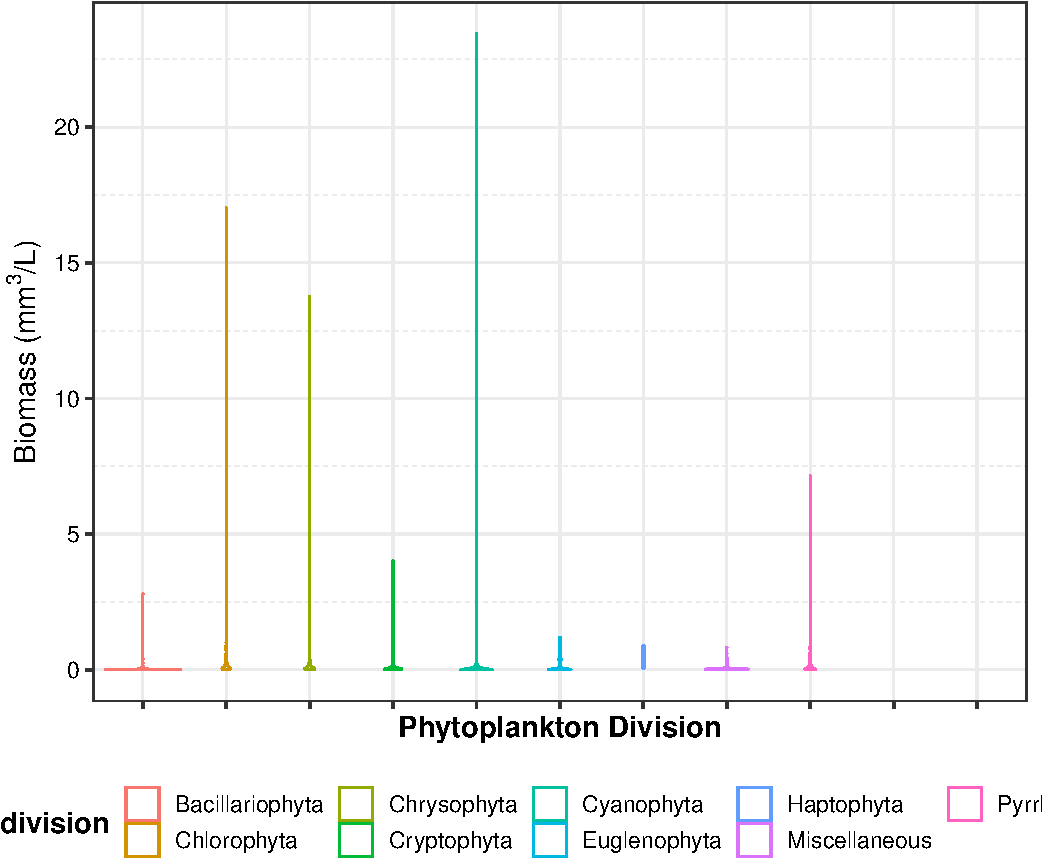
\includegraphics{Chen_ENV872_Project_files/figure-latex/Figure 1-1.pdf}

\begin{verbatim}
## `geom_smooth()` using method = 'loess' and formula 'y ~ x'
\end{verbatim}

\begin{verbatim}
## Warning: Removed 28 rows containing non-finite values (stat_smooth).
\end{verbatim}

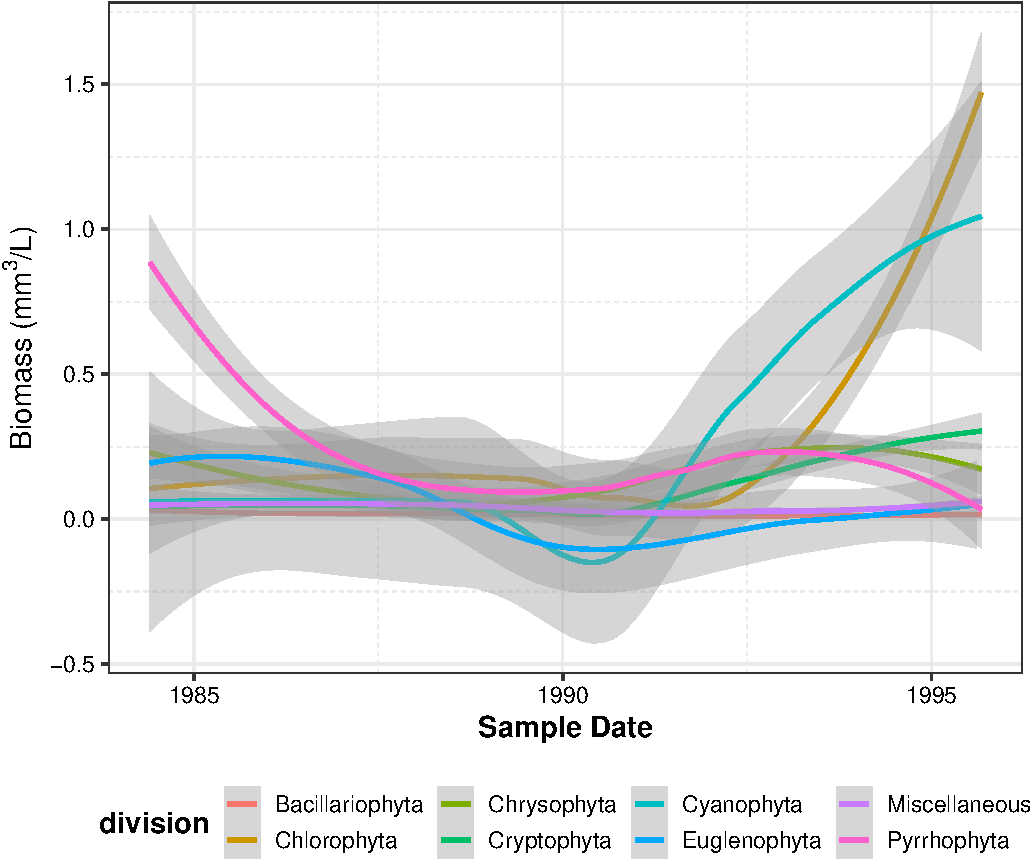
\includegraphics{Chen_ENV872_Project_files/figure-latex/Figure 2-1.pdf}

\begin{verbatim}
## Warning: Removed 65 rows containing non-finite values (stat_boxplot).
\end{verbatim}

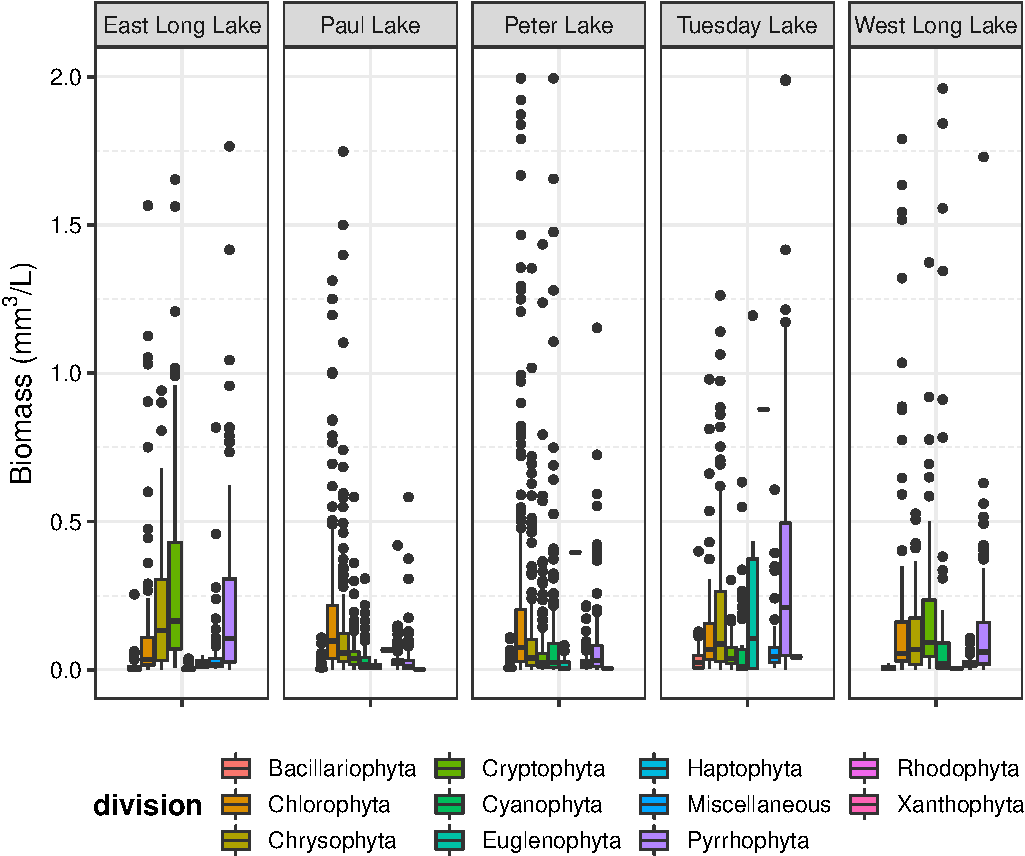
\includegraphics{Chen_ENV872_Project_files/figure-latex/Figure 3-1.pdf}
\newpage

\section{Analysis}\label{analysis}

\begin{Shaded}
\begin{Highlighting}[]
\CommentTok{# Evaluate assumption of normal distribution}
\KeywordTok{shapiro.test}\NormalTok{(biomass_nutrients}\OperatorTok{$}\NormalTok{tot_biomass) }\CommentTok{# less than 0.05, not normally distributed}
\end{Highlighting}
\end{Shaded}

\begin{verbatim}
## 
##  Shapiro-Wilk normality test
## 
## data:  biomass_nutrients$tot_biomass
## W = 0.51532, p-value < 2.2e-16
\end{verbatim}

\begin{Shaded}
\begin{Highlighting}[]
\KeywordTok{qqnorm}\NormalTok{(biomass_nutrients}\OperatorTok{$}\NormalTok{tot_biomass); }\KeywordTok{qqline}\NormalTok{(biomass_nutrients}\OperatorTok{$}\NormalTok{tot_biomass)}
\end{Highlighting}
\end{Shaded}

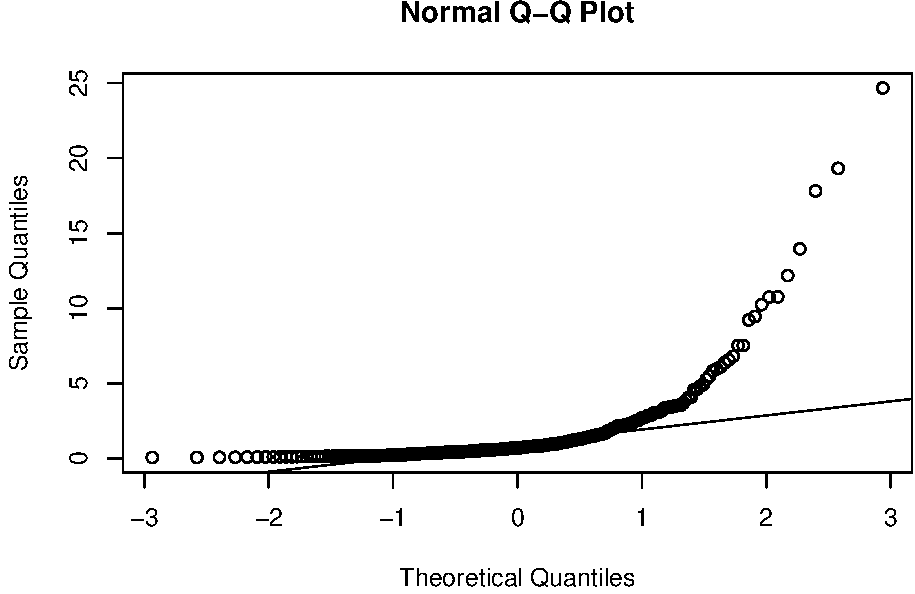
\includegraphics{Chen_ENV872_Project_files/figure-latex/Analysis-1.pdf}

\begin{Shaded}
\begin{Highlighting}[]
\CommentTok{#}
\end{Highlighting}
\end{Shaded}

\newpage

\section{Summary and Conclusions}\label{summary-and-conclusions}

Overall,


\end{document}
